\PassOptionsToPackage{unicode=true}{hyperref} % options for packages loaded elsewhere
\PassOptionsToPackage{hyphens}{url}
%
\documentclass[ignorenonframetext,]{beamer}
\usepackage{pgfpages}
\setbeamertemplate{caption}[numbered]
\setbeamertemplate{caption label separator}{: }
\setbeamercolor{caption name}{fg=normal text.fg}
\beamertemplatenavigationsymbolsempty
% Prevent slide breaks in the middle of a paragraph:
\widowpenalties 1 10000
\raggedbottom
\setbeamertemplate{part page}{
\centering
\begin{beamercolorbox}[sep=16pt,center]{part title}
  \usebeamerfont{part title}\insertpart\par
\end{beamercolorbox}
}
\setbeamertemplate{section page}{
\centering
\begin{beamercolorbox}[sep=12pt,center]{part title}
  \usebeamerfont{section title}\insertsection\par
\end{beamercolorbox}
}
\setbeamertemplate{subsection page}{
\centering
\begin{beamercolorbox}[sep=8pt,center]{part title}
  \usebeamerfont{subsection title}\insertsubsection\par
\end{beamercolorbox}
}
\AtBeginPart{
  \frame{\partpage}
}
%\AtBeginSection{
%  \ifbibliography
%  \else
%    \frame{\sectionpage}
%  \fi
%}
\AtBeginSubsection{
  \frame{\subsectionpage}
}
\usepackage{lmodern}
\usepackage{amssymb,amsmath}
\usepackage{ifxetex,ifluatex}
\usepackage{fixltx2e} % provides \textsubscript
\ifnum 0\ifxetex 1\fi\ifluatex 1\fi=0 % if pdftex
  \usepackage[T1]{fontenc}
  \usepackage[utf8]{inputenc}
  \usepackage{textcomp} % provides euro and other symbols
\else % if luatex or xelatex
  \usepackage{unicode-math}
  \defaultfontfeatures{Ligatures=TeX,Scale=MatchLowercase}
\fi
\usetheme[]{PaloAlto}
\usecolortheme{orchid}
% use upquote if available, for straight quotes in verbatim environments
\IfFileExists{upquote.sty}{\usepackage{upquote}}{}
% use microtype if available
\IfFileExists{microtype.sty}{%
\usepackage[]{microtype}
\UseMicrotypeSet[protrusion]{basicmath} % disable protrusion for tt fonts
}{}
\IfFileExists{parskip.sty}{%
\usepackage{parskip}
}{% else
\setlength{\parindent}{0pt}
\setlength{\parskip}{6pt plus 2pt minus 1pt}
}
\usepackage{hyperref}
\hypersetup{
            pdfauthor={Anthony Raborn\^{}1; Walter Leite; Katerina Marcoulides},
            pdfborder={0 0 0},
            breaklinks=true}
\urlstyle{same}  % don't use monospace font for urls
\newif\ifbibliography
\usepackage{graphicx,grffile}
\makeatletter
\def\maxwidth{\ifdim\Gin@nat@width>\linewidth\linewidth\else\Gin@nat@width\fi}
\def\maxheight{\ifdim\Gin@nat@height>\textheight\textheight\else\Gin@nat@height\fi}
\makeatother
% Scale images if necessary, so that they will not overflow the page
% margins by default, and it is still possible to overwrite the defaults
% using explicit options in \includegraphics[width, height, ...]{}
\setkeys{Gin}{width=\maxwidth,height=\maxheight,keepaspectratio}
\setlength{\emergencystretch}{3em}  % prevent overfull lines
\providecommand{\tightlist}{%
  \setlength{\itemsep}{0pt}\setlength{\parskip}{0pt}}
\setcounter{secnumdepth}{0}

% set default figure placement to htbp
\makeatletter
\def\fps@figure{htbp}
\makeatother

\usepackage{booktabs}
\usepackage{longtable}
\usepackage{array}
\usepackage{multirow}
\usepackage{wrapfig}
\usepackage{float}
\usepackage{colortbl}
\usepackage{pdflscape}
\usepackage{tabu}
\usepackage{threeparttable}
\usepackage{threeparttablex}
\usepackage[normalem]{ulem}
\usepackage{makecell}
\usepackage{caption}

\title{Comparison of Automated Short Form Selection Strategies}
\author{Anthony Raborn\(^1\) \and Walter Leite \and Katerina Marcoulides}
\providecommand{\institute}[1]{}
\institute{Research and Evaluation Methodology Department \and University of Florida \and 1:
\href{mailto:anthony.w.raborn@gmail.com}{\nolinkurl{anthony.w.raborn@gmail.com}}}
\date{November 14, 2018}

\begin{document}
\frame{\titlepage}

\hypertarget{introduction}{%
\section{Introduction}\label{introduction}}

\begin{frame}{Applications of Psychometric Scales}
\protect\hypertarget{applications-of-psychometric-scales}{}

Applied researchers are often faced with a dilemma, both with drawbacks:

\begin{enumerate}[A]
  \item Use a well-established but lengthy scale \\
    -- Potentially longer administration time for less information
  \item Use a few items from a scale \\
    -- Potentially greater information but weaker validity evidence
\end{enumerate}

In the literature, researchers attempt to use Option B with some effort
spent on collecting validity evidence

\end{frame}

\begin{frame}{Examples of Item Selection Methods for Short Forms}
\protect\hypertarget{examples-of-item-selection-methods-for-short-forms}{}

\begin{enumerate}
\tightlist
\item
  Hand-Selecting Items
\end{enumerate}

\begin{itemize}
\tightlist
\item
  Using theoretical or practical justifications per item (e.g., Noble,
  Jensen, Naylor, Bhullar, \& Akeroyd, 2013)
\item
  Retaining one of many (qualitatively) redundant items (e.g., Dennis,
  2003)
\end{itemize}

\begin{enumerate}
\setcounter{enumi}{1}
\tightlist
\item
  Statistical Criteria
\end{enumerate}

\begin{itemize}
\tightlist
\item
  Retaining items with high factor loadings or item correlations (e.g.,
  Byrne \& Pachana, 2011; Wester, Vogel, O'neil, \& Danforth, 2012)
\item
  Selecting items that improve measures of reliability and/or
  dimensionality (e.g., Lim \& Chapman, 2013; Veale, 2014)
\end{itemize}

\end{frame}

\begin{frame}{Problem}
\protect\hypertarget{problem}{}

Creating short forms with (1) good internal structure and (2) good
predictive, convergent, and/or divergent validity is difficult by hand
using \emph{any} criteria.

One potential solution would be to use metaheuristic optimization
algorithms (Dréo, Pétrowski, Siarry, \& Taillard, 2006).

\end{frame}

\begin{frame}{Goals of this Study}
\protect\hypertarget{goals-of-this-study}{}

\begin{itemize}
\tightlist
\item
  Compare different automatic scale reduction strategies

  \begin{enumerate}
  \tightlist
  \item
    Model fit of final scales (better fit is better)
  \item
    Removal of specific problematic items (fewer problematic items is
    better)
  \item
    Reliability of final scales (higher reliability is better)
  \item
    Time to converge (faster is better)
  \end{enumerate}
\item
  Determine which factors affect these comparisons

  \begin{enumerate}
  \tightlist
  \item
    Population model type (one factor, three factor)
  \item
    Severity of problematic items (none, minor, major)
  \item
    Strength of relationship to external criterion (none, moderate)
  \end{enumerate}
\end{itemize}

\end{frame}

\hypertarget{theoretical-framework}{%
\section{Theoretical Framework}\label{theoretical-framework}}

\begin{frame}{Previous Attempts}
\protect\hypertarget{previous-attempts}{}

Some ``common'' algorithms in the literature:

\begin{enumerate}
\tightlist
\item
  ``Maximize Main Loadings'' (not investigated)
\item
  Ant Colony Optimization (ACO)
\item
  Tabu Search (TS)
\item
  Genetic Algorithm (GA)
\end{enumerate}

An additional method investigated in this study:

\begin{enumerate}
\setcounter{enumi}{4}
\tightlist
\item
  Simulated Annealing (SA)
\end{enumerate}

\end{frame}

\hypertarget{method}{%
\section{Method}\label{method}}

\begin{frame}{Factors Manipulated}
\protect\hypertarget{factors-manipulated}{}

\begin{enumerate}
\tightlist
\item
  The dimensionality of the full form
\end{enumerate}

\begin{itemize}
\tightlist
\item
  One Factor
\item
  Three Factor
\end{itemize}

\begin{enumerate}
\setcounter{enumi}{1}
\tightlist
\item
  Full-scale model misspecification
\end{enumerate}

\begin{itemize}
\tightlist
\item
  No misspecification
\item
  Minor misspecification (six items loading on a nuisance parameter with
  \(\lambda=.3\))
\item
  Major misspecification (six items loading on a nuisance parameter with
  \(\lambda=.6\))
\end{itemize}

\begin{enumerate}
\setcounter{enumi}{2}
\tightlist
\item
  Relationship to External Criterion Variable
\end{enumerate}

\begin{itemize}
\tightlist
\item
  No relationship
\item
  Moderate relationship (\(\gamma = .6\))
\end{itemize}

\end{frame}

\begin{frame}{One Factor Model}
\protect\hypertarget{one-factor-model}{}

\begin{figure}
\centering
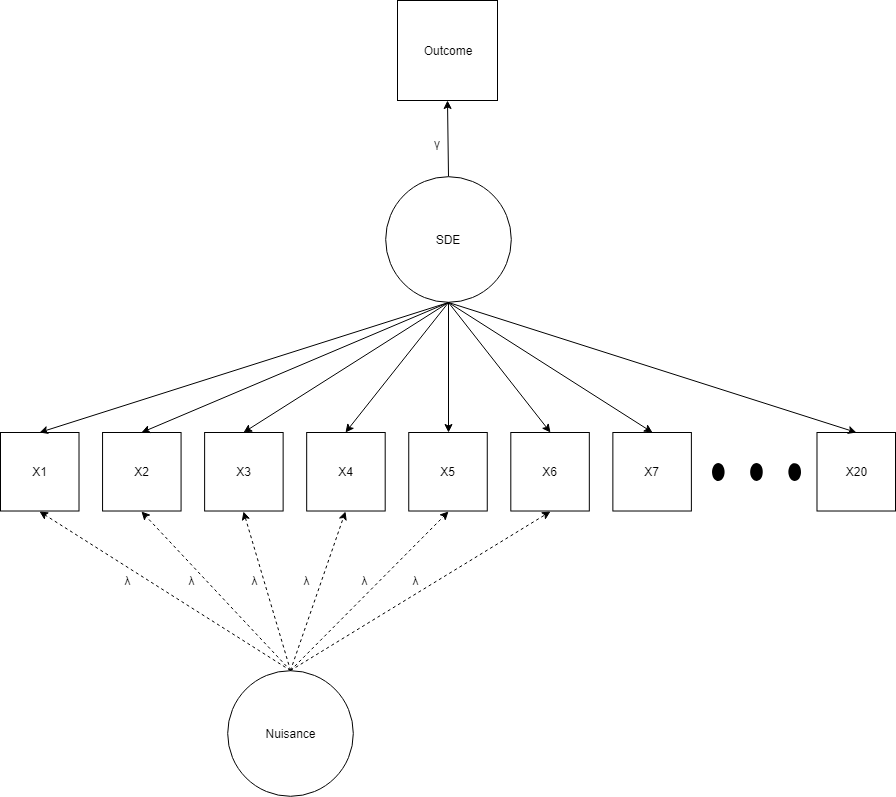
\includegraphics[width=2.86458in,height=\textheight]{Factor Diagrams/One Factor Diagram.png}
\caption{20-item Self-Deceptive Enhancement Scale (Leite \& Beretvas,
2005)}
\end{figure}

\end{frame}

\begin{frame}{Three Factor Model}
\protect\hypertarget{three-factor-model}{}

\begin{figure}
\centering
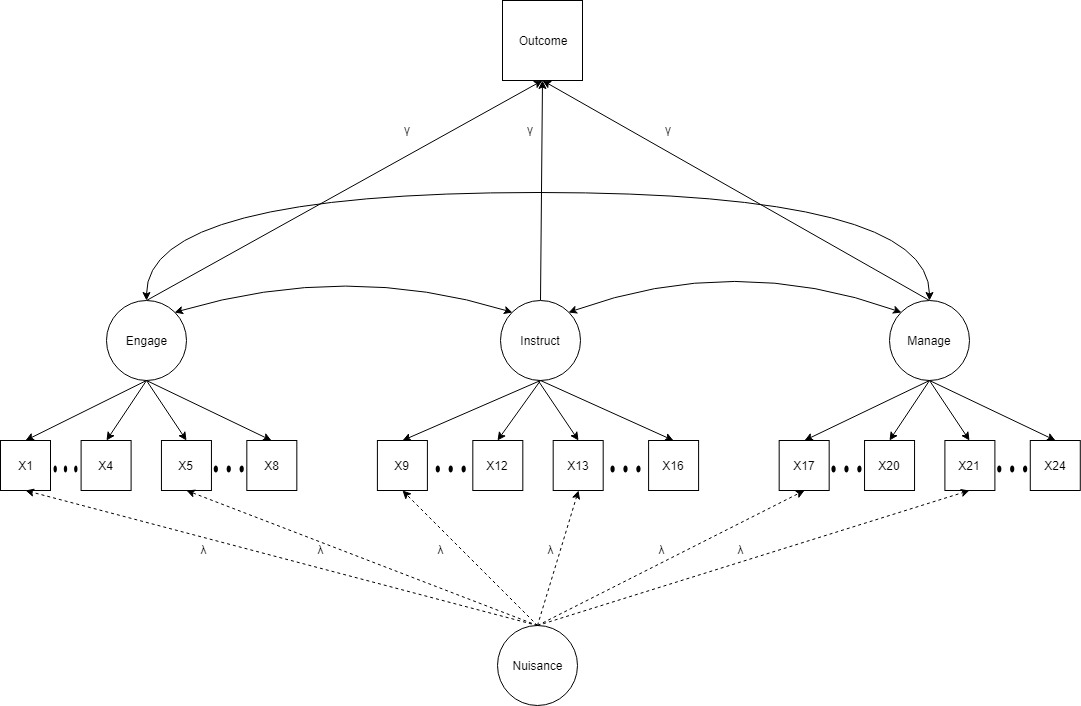
\includegraphics[width=3.85417in,height=\textheight]{Factor Diagrams/Three Factor Diagram.png}
\caption{24-item Teacher Efficacy Scale (Tschannen-Moran \& Hoy, 2001)}
\end{figure}

\end{frame}

\begin{frame}[fragile]{Simulation}
\protect\hypertarget{simulation}{}

Program: R (R Core Team, 2018)

Packages:

\begin{enumerate}
\tightlist
\item
  \texttt{MASS} (Venables \& Ripley, 2002) (data simulation)
\item
  \texttt{ShortForm} (Raborn \& Leite, 2018) (ACO, SA, TS)
\item
  \texttt{GAabbreviate} (Sahdra et al., 2016) (GA; modified)
\end{enumerate}

Sample Size: \(n = 500\)

Iterations: 100

\end{frame}

\begin{frame}{Analysis of Results}
\protect\hypertarget{analysis-of-results}{}

\begin{enumerate}
\tightlist
\item
  CFI, TLI, RMSEA
\item
  Proportion of iterations including each problematic item (excluding no
  error condition)
\item
  Composite reliability of each factor:
  \[CR_{factor} = \frac{(\Sigma^I_{i=1}Loading_i)^2}{(\Sigma^I_{i=1}Loading_i)^2 + \Sigma^I_{i=1}(Residual^2_i)} \]
\item
  Run time of algorithms
\end{enumerate}

\end{frame}

\hypertarget{results}{%
\section{Results}\label{results}}

\begin{frame}{One Factor Model Fit: No External Variable}
\protect\hypertarget{one-factor-model-fit-no-external-variable}{}

\begin{table}[H]
\centering
\resizebox{\linewidth}{!}{
\begin{tabular}{>{\raggedright\arraybackslash}p{0.7in}>{\raggedright\arraybackslash}p{0.7in}>{\raggedright\arraybackslash}p{0.7in}>{\raggedright\arraybackslash}p{0.7in}>{\raggedright\arraybackslash}p{0.7in}>{}p{0.7in}>{}p{0.7in}}
\toprule
Error Condition & Method & CFI & TLI & RMSEA\\
\midrule
 & ACO & \textbf{0.975} & \textbf{0.967} & \textbf{0.045}\\

 & SA & \textbf{0.992} & \textbf{0.990} & \textbf{0.020}\\

 & TS & \textbf{0.985} & \textbf{0.981} & \textbf{0.027}\\

\multirow{-4}{0.7in}{\raggedright\arraybackslash None} & GA & \textbf{0.975} & \textbf{0.968} & \textbf{0.043}\\
\cmidrule{1-5}
 & ACO & \textbf{0.966} & \textbf{0.956} & 0.052\\

 & SA & \textbf{0.989} & \textbf{0.987} & \textbf{0.022}\\

 & TS & \textbf{0.978} & \textbf{0.972} & \textbf{0.035}\\

\multirow{-4}{0.7in}{\raggedright\arraybackslash Minor} & GA & \textbf{0.968} & \textbf{0.959} & \textbf{0.048}\\
\cmidrule{1-5}
 & ACO & 0.944 & 0.928 & 0.062\\

 & SA & \textbf{0.983} & \textbf{0.979} & \textbf{0.028}\\

 & TS & 0.944 & 0.928 & 0.057\\

\multirow{-4}{0.7in}{\raggedright\arraybackslash Major} & GA & 0.846 & 0.802 & 0.113\\
\bottomrule
\end{tabular}}
\end{table}

\end{frame}

\begin{frame}{One Factor Model Fit: External Variable}
\protect\hypertarget{one-factor-model-fit-external-variable}{}

\small
\begin{table}[H]
\centering
\resizebox{\linewidth}{!}{
\begin{tabular}{>{\raggedright\arraybackslash}p{1in}>{\raggedright\arraybackslash}p{1in}>{\raggedright\arraybackslash}p{1in}>{\raggedright\arraybackslash}p{1in}>{\raggedright\arraybackslash}p{1in}l}
\toprule
Error Condition & External Relationship & Method & CFI & TLI & RMSEA\\
\midrule
\addlinespace[0.3em]
\multicolumn{6}{l}{\textbf{None}}\\
 & None & ACO & \textbf{0.975} & \textbf{0.967} & \textbf{0.045}\\

 & None & SA & \textbf{0.992} & \textbf{0.990} & \textbf{0.020}\\

 & None & TS & \textbf{0.985} & \textbf{0.981} & \textbf{0.027}\\

\multirow{-4}{1in}{\raggedright\arraybackslash \hspace{1em}} & None & GA & \textbf{0.975} & \textbf{0.968} & \textbf{0.043}\\
\cmidrule{1-6}
 & Moderate & ACO & \textbf{0.979} & \textbf{0.973} & \textbf{0.040}\\

 & Moderate & SA & \textbf{0.991} & \textbf{0.989} & \textbf{0.021}\\

 & Moderate & TS & \textbf{0.985} & \textbf{0.981} & \textbf{0.027}\\

\multirow{-4}{1in}{\raggedright\arraybackslash \hspace{1em}} & Moderate & GA & \textbf{0.975} & \textbf{0.968} & \textbf{0.044}\\
\cmidrule{1-6}
\addlinespace[0.3em]
\multicolumn{6}{l}{\textbf{Major}}\\
 & None & ACO & 0.944 & 0.928 & 0.062\\

 & None & SA & \textbf{0.983} & \textbf{0.979} & \textbf{0.028}\\

 & None & TS & 0.944 & 0.928 & 0.057\\

\multirow{-4}{1in}{\raggedright\arraybackslash \hspace{1em}} & None & GA & 0.846 & 0.802 & 0.113\\
\cmidrule{1-6}
 & Moderate & ACO & 0.945 & 0.931 & 0.058\\

 & Moderate & SA & \textbf{0.981} & \textbf{0.977} & \textbf{0.029}\\

 & Moderate & TS & 0.930 & 0.912 & 0.063\\

\multirow{-4}{1in}{\raggedright\arraybackslash \hspace{1em}} & Moderate & GA & 0.858 & 0.822 & 0.107\\
\bottomrule
\end{tabular}}
\end{table}

\end{frame}

\begin{frame}{One Factor Item Selection Proportions: No External
Variable}
\protect\hypertarget{one-factor-item-selection-proportions-no-external-variable}{}

\begin{table}[H]
\centering
\resizebox{\linewidth}{!}{
\begin{tabular}{lllllll}
\toprule
Error Condition & Item & Factor Loading & ACO & SA & TS & GA\\
\midrule
 & y3 & 0.580 & 0.84 & 0.39 & 0.48 & 0.66\\

 & y5 & 0.534 & 0.81 & 0.36 & 0.43 & 0.35\\

 & y4 & 0.448 & 0.70 & 0.59 & 0.53 & 0.61\\

 & y2 & 0.408 & 0.66 & 0.36 & 0.37 & 0.41\\

 & y6 & 0.393 & 0.51 & 0.38 & 0.39 & 0.93\\

\multirow{-6}{*}{\raggedright\arraybackslash Minor} & y1 & 0.382 & 0.34 & 0.39 & 0.48 & 0.48\\
\cmidrule{1-7}
 & y3 & 0.580 & 0.49 & 0.12 & 0.46 & 0.61\\

 & y5 & 0.534 & 0.35 & 0.32 & 0.48 & 0.44\\

 & y4 & 0.448 & 0.33 & 0.17 & 0.48 & 0.70\\

 & y2 & 0.408 & 0.19 & 0.19 & 0.37 & 0.48\\

 & y6 & 0.393 & 0.21 & 0.21 & 0.36 & 0.96\\

\multirow{-6}{*}{\raggedright\arraybackslash Major} & y1 & 0.382 & 0.21 & 0.21 & 0.48 & 0.44\\
\cmidrule{1-7}
\textbf{Minor Error Average Proportion:} & \textbf{} & \textbf{} & \textbf{0.643} & \textbf{0.412} & \textbf{0.447} & \textbf{0.573}\\
\cmidrule{1-7}
\textbf{Major Error Average Proportion:} & \textbf{} & \textbf{} & \textbf{0.297} & \textbf{0.203} & \textbf{0.438} & \textbf{0.605}\\
\bottomrule
\end{tabular}}
\end{table}

\end{frame}

\begin{frame}{One Factor Item Selection Proportions: External Variable}
\protect\hypertarget{one-factor-item-selection-proportions-external-variable}{}

\begin{table}[H]
\centering
\resizebox{\linewidth}{!}{
\begin{tabular}{llllllll}
\toprule
Error Condition & External Condition & Item & Factor Loading & ACO & SA & TS & GA\\
\midrule
 & None & y3 & 0.580 & 0.78 & 0.48 & 0.46 & 0.82\\

 & None & y5 & 0.534 & 0.75 & 0.39 & 0.47 & 0.98\\

 & None & y4 & 0.448 & 0.65 & 0.45 & 0.50 & 0.21\\

 & None & y2 & 0.408 & 0.34 & 0.34 & 0.41 & 0.29\\

 & None & y6 & 0.393 & 0.29 & 0.55 & 0.55 & 0.29\\

\multirow{-6}{*}{\raggedright\arraybackslash Major} & None & y1 & 0.382 & 0.16 & 0.48 & 0.51 & 0.18\\
\cmidrule{1-8}
 & Moderate & y3 & 0.580 & 0.49 & 0.10 & 0.44 & 0.80\\

 & Moderate & y5 & 0.534 & 0.17 & 0.13 & 0.42 & 0.98\\

 & Moderate & y4 & 0.448 & 0.16 & 0.13 & 0.38 & 0.26\\

 & Moderate & y2 & 0.408 & 0.12 & 0.14 & 0.47 & 0.43\\

 & Moderate & y6 & 0.393 & 0.16 & 0.20 & 0.40 & 0.43\\

\multirow{-6}{*}{\raggedright\arraybackslash Major} & Moderate & y1 & 0.382 & 0.15 & 0.24 & 0.53 & 0.46\\
\cmidrule{1-8}
\textbf{} & \textbf{No External Average Proportion:} & \textbf{} & \textbf{} & \textbf{0.495} & \textbf{0.448} & \textbf{0.483} & \textbf{0.462}\\
\cmidrule{1-8}
\textbf{} & \textbf{Moderate External Average Proportion:} & \textbf{} & \textbf{} & \textbf{0.208} & \textbf{0.157} & \textbf{0.440} & \textbf{0.560}\\
\bottomrule
\end{tabular}}
\end{table}

\end{frame}

\begin{frame}{Three Factor Model Fit: No External Variable}
\protect\hypertarget{three-factor-model-fit-no-external-variable}{}

\begin{table}[H]
\centering
\resizebox{\linewidth}{!}{
\begin{tabular}{>{\raggedright\arraybackslash}p{0.7in}>{\raggedright\arraybackslash}p{0.7in}>{\raggedright\arraybackslash}p{0.7in}>{\raggedright\arraybackslash}p{0.7in}>{\raggedright\arraybackslash}p{0.7in}}
\toprule
Error Condition & Method & CFI & TLI & RMSEA\\
\midrule
 & ACO & \textbf{0.980} & \textbf{0.974} & \textbf{0.042}\\

 & SA & \textbf{0.992} & \textbf{0.990} & \textbf{0.023}\\

 & TS & \textbf{0.989} & \textbf{0.986} & \textbf{0.027}\\

\multirow{-4}{0.7in}{\raggedright\arraybackslash None} & GA & \textbf{0.979} & \textbf{0.973} & \textbf{0.042}\\
\cmidrule{1-5}
 & ACO & \textbf{0.972} & \textbf{0.964} & \textbf{0.050}\\

 & SA & \textbf{0.990} & \textbf{0.987} & \textbf{0.026}\\

 & TS & \textbf{0.984} & \textbf{0.979} & \textbf{0.035}\\

\multirow{-4}{0.7in}{\raggedright\arraybackslash Minor} & GA & \textbf{0.970} & \textbf{0.961} & \textbf{0.050}\\
\cmidrule{1-5}
 & ACO & \textbf{0.953} & 0.939 & 0.062\\

 & SA & \textbf{0.989} & \textbf{0.986} & \textbf{0.027}\\

 & TS & \textbf{0.961} & \textbf{0.950} & 0.053\\

\multirow{-4}{0.7in}{\raggedright\arraybackslash Major} & GA & 0.909 & 0.882 & 0.089\\
\bottomrule
\end{tabular}}
\end{table}

\end{frame}

\begin{frame}{Three Factor Model Fit: External Variable}
\protect\hypertarget{three-factor-model-fit-external-variable}{}

\begin{table}[H]
\centering
\resizebox{\linewidth}{!}{
\begin{tabular}{>{\raggedright\arraybackslash}p{1in}>{\raggedright\arraybackslash}p{1in}>{\raggedright\arraybackslash}p{1in}>{\raggedright\arraybackslash}p{1in}>{\raggedright\arraybackslash}p{1in}l}
\toprule
Error Condition & External Relationship & Method & CFI & TLI & RMSEA\\
\midrule
\addlinespace[0.3em]
\multicolumn{6}{l}{\textbf{None}}\\
 & None & ACO & \textbf{0.980} & \textbf{0.974} & \textbf{0.042}\\

 & None & SA & \textbf{0.992} & \textbf{0.990} & \textbf{0.023}\\

 & None & TS & \textbf{0.989} & \textbf{0.986} & \textbf{0.027}\\

\multirow{-4}{1in}{\raggedright\arraybackslash \hspace{1em}} & None & GA & \textbf{0.979} & \textbf{0.973} & \textbf{0.042}\\
\cmidrule{1-6}
 & Moderate & ACO & \textbf{0.977} & \textbf{0.970} & \textbf{0.047}\\

 & Moderate & SA & \textbf{0.988} & \textbf{0.984} & \textbf{0.032}\\

 & Moderate & TS & \textbf{0.983} & \textbf{0.978} & \textbf{0.037}\\

\multirow{-4}{1in}{\raggedright\arraybackslash \hspace{1em}} & Moderate & GA & \textbf{0.977} & \textbf{0.970} & \textbf{0.046}\\
\cmidrule{1-6}
\addlinespace[0.3em]
\multicolumn{6}{l}{\textbf{Major}}\\
 & None & ACO & \textbf{0.953} & 0.939 & 0.062\\

 & None & SA & \textbf{0.989} & \textbf{0.986} & \textbf{0.027}\\

 & None & TS & \textbf{0.961} & \textbf{0.950} & 0.053\\

\multirow{-4}{1in}{\raggedright\arraybackslash \hspace{1em}} & None & GA & 0.909 & 0.882 & 0.089\\
\cmidrule{1-6}
 & Moderate & ACO & \textbf{0.964} & \textbf{0.953} & 0.057\\

 & Moderate & SA & \textbf{0.984} & \textbf{0.979} & \textbf{0.036}\\

 & Moderate & TS & \textbf{0.953} & 0.939 & 0.061\\

\multirow{-4}{1in}{\raggedright\arraybackslash \hspace{1em}} & Moderate & GA & 0.907 & 0.880 & 0.091\\
\bottomrule
\end{tabular}}
\end{table}

\end{frame}

\begin{frame}{Three Factor Item Selection Proportions: No External
Variable}
\protect\hypertarget{three-factor-item-selection-proportions-no-external-variable}{}

\begin{table}[H]
\centering
\resizebox{\linewidth}{!}{
\begin{tabular}{lllllll}
\toprule
Error Condition & Item & Factor Loading & ACO & SA & TS & GA\\
\midrule
 & y1 & 0.9 & 0.83 & 0.36 & 0.49 & 0.94\\

 & y5 & 0.7 & 0.13 & 0.58 & 0.50 & 0.24\\

 & y9 & 0.9 & 0.52 & 0.34 & 0.41 & 0.87\\

 & y13 & 0.7 & 0.20 & 0.42 & 0.48 & 0.08\\

 & y17 & 0.9 & 0.85 & 0.25 & 0.28 & 0.65\\

\multirow{-6}{*}{\raggedright\arraybackslash Minor} & y21 & 0.7 & 0.45 & 0.36 & 0.44 & 0.39\\
\cmidrule{1-7}
 & y1 & 0.9 & 0.60 & 0.32 & 0.44 & 0.90\\

 & y5 & 0.7 & 0.22 & 0.22 & 0.41 & 0.12\\

 & y9 & 0.9 & 0.20 & 0.12 & 0.24 & 0.97\\

 & y13 & 0.7 & 0.10 & 0.11 & 0.32 & 0.03\\

 & y17 & 0.9 & 0.61 & 0.10 & 0.30 & 0.60\\

\multirow{-6}{*}{\raggedright\arraybackslash Major} & y21 & 0.7 & 0.30 & 0.10 & 0.27 & 0.41\\
\cmidrule{1-7}
\textbf{Minor Error Average Proportion:} & \textbf{} & \textbf{} & \textbf{0.497} & \textbf{0.385} & \textbf{0.433} & \textbf{0.528}\\
\cmidrule{1-7}
\textbf{Major Error Average Proportion:} & \textbf{} & \textbf{} & \textbf{0.338} & \textbf{0.162} & \textbf{0.330} & \textbf{0.505}\\
\bottomrule
\end{tabular}}
\end{table}

\end{frame}

\begin{frame}{Three Factor Item Selection Proportions: External
Variable}
\protect\hypertarget{three-factor-item-selection-proportions-external-variable}{}

\begin{table}[H]
\centering
\resizebox{\linewidth}{!}{
\begin{tabular}{llllllll}
\toprule
Error Condition & External Condition & Item & Factor Loading & ACO & SA & TS & GA\\
\midrule
 & None & y1 & 0.9 & 0.60 & 0.32 & 0.44 & 0.90\\

 & None & y5 & 0.7 & 0.22 & 0.22 & 0.41 & 0.12\\

 & None & y9 & 0.9 & 0.20 & 0.12 & 0.24 & 0.97\\

 & None & y13 & 0.7 & 0.10 & 0.11 & 0.32 & 0.03\\

 & None & y17 & 0.9 & 0.61 & 0.10 & 0.30 & 0.60\\

\multirow{-6}{*}{\raggedright\arraybackslash Major} & None & y21 & 0.7 & 0.30 & 0.10 & 0.27 & 0.41\\
\cmidrule{1-8}
 & Moderate & y1 & 0.9 & 0.37 & 0.25 & 0.51 & 0.84\\

 & Moderate & y5 & 0.7 & 0.15 & 0.12 & 0.37 & 0.16\\

 & Moderate & y9 & 0.9 & 0.32 & 0.16 & 0.30 & 0.97\\

 & Moderate & y13 & 0.7 & 0.06 & 0.16 & 0.20 & 0.03\\

 & Moderate & y17 & 0.9 & 0.29 & 0.10 & 0.37 & 0.96\\

\multirow{-6}{*}{\raggedright\arraybackslash Major} & Moderate & y21 & 0.7 & 0.04 & 0.09 & 0.37 & 0.04\\
\cmidrule{1-8}
\textbf{} & \textbf{No External Average Proportion:} & \textbf{} & \textbf{} & \textbf{0.338} & \textbf{0.162} & \textbf{0.330} & \textbf{0.505}\\
\cmidrule{1-8}
\textbf{} & \textbf{Moderate External Average Proportion:} & \textbf{} & \textbf{} & \textbf{0.205} & \textbf{0.147} & \textbf{0.353} & \textbf{0.500}\\
\bottomrule
\end{tabular}}
\end{table}

\end{frame}

\hypertarget{discussion}{%
\section{Discussion}\label{discussion}}

\begin{frame}{Best Performing Methods}
\protect\hypertarget{best-performing-methods}{}

\begin{enumerate}
\tightlist
\item
  Removal of specific problematic items: \textbf{SA}
\item
  Model fit of final scales: \textbf{SA}
\item
  Reliability of final scales: About equivalent (\emph{ACO} somewhat
  higher)
\item
  Time to converge: About equivalent (\emph{TS} one factor longer)
\end{enumerate}

Overall: SA consistently had good\footnote<.->{CFI \textgreater{} .95,
  TLI \textgreater{} .95, RMSEA \textless{} .05} fit; ACO \& TS
consistently had at least adequate\footnote<.->{CFI \textgreater{} .90,
  TLI \textgreater{} .90, RMSEA \textless{} .08} fit; GA produced poor
fit in the presence of major error

\end{frame}

\begin{frame}{Factors Affecting Comparisons}
\protect\hypertarget{factors-affecting-comparisons}{}

\small
\begin{enumerate}
   \item Population model type\\
      -- model fit: one factor < three factor\\
      -- Minimal effect on time to converge
  \item Severity of problematic items\\
      -- Decreased model fit, \textbf{SA} excluded
  \item  Strength of relationship to external criterion\\
      -- Somewhat attenuates effect of error only for \textbf{ACO}
\end{enumerate}

\end{frame}

\begin{frame}{For the Future}
\protect\hypertarget{for-the-future}{}

\begin{block}{Suggestions for Applied Researchers}

\begin{enumerate}[A]
  \item Apply each algorithm to your sample--grab some coffee or tea while they each run!
  \item Compare the resulting short forms against one another ("face validity" comparisons).
  \item When possible, test against a second sample (cross-validation).
\end{enumerate}

\end{block}

\begin{block}{Future Research Questions}

\begin{enumerate}
\tightlist
\item
  How well do the short forms created by each algorithm generalize to
  new samples?
\item
  How do additional manipulations (e.g., population models, types of
  errors) affect the algorithms?
\end{enumerate}

\end{block}

\end{frame}

\begin{frame}{Corresponding Author}
\protect\hypertarget{corresponding-author}{}

\center{\huge{anthony.w.raborn@gmail.com}}

\end{frame}

\hypertarget{references}{%
\section{References}\label{references}}

\begin{frame}[allowframebreaks]{References}
\protect\hypertarget{references-1}{}

\tiny

\hypertarget{refs}{}
\leavevmode\hypertarget{ref-byrne2011development}{}%
Byrne, G. J., \& Pachana, N. A. (2011). Development and validation of a
short form of the geriatric anxiety inventory--the gai-sf.
\emph{International Psychogeriatrics}, \emph{23}(1), 125--131.

\leavevmode\hypertarget{ref-dennis2003breastfeeding}{}%
Dennis, C.-L. (2003). The breastfeeding self-efficacy scale:
Psychometric assessment of the short form. \emph{Journal of Obstetric,
Gynecologic, \& Neonatal Nursing}, \emph{32}(6), 734--744.

\leavevmode\hypertarget{ref-dreo2006metaheuristics}{}%
Dréo, J., Pétrowski, A., Siarry, P., \& Taillard, E. (2006).
\emph{Metaheuristics for hard optimization: Methods and case studies}.
Springer Science \& Business Media.

\leavevmode\hypertarget{ref-leite2005validation}{}%
Leite, W. L., \& Beretvas, S. N. (2005). Validation of scores on the
marlowe-crowne social desirability scale and the balanced inventory of
desirable responding. \emph{Educational and Psychological Measurement},
\emph{65}(1), 140--154.

\leavevmode\hypertarget{ref-lim2013development}{}%
Lim, S. Y., \& Chapman, E. (2013). Development of a short form of the
attitudes toward mathematics inventory. \emph{Educational Studies in
Mathematics}, \emph{82}(1), 145--164.

\leavevmode\hypertarget{ref-noble2013short}{}%
Noble, W., Jensen, N. S., Naylor, G., Bhullar, N., \& Akeroyd, M. A.
(2013). A short form of the speech, spatial and qualities of hearing
scale suitable for clinical use: The ssq12. \emph{International Journal
of Audiology}, \emph{52}(6), 409--412.

\leavevmode\hypertarget{ref-Raborn2018}{}%
Raborn, A., \& Leite, W. (2018). \emph{ShortForm: Automatic short form
creation}. Retrieved from
\url{https://github.com/AnthonyRaborn/ShortForm}

\leavevmode\hypertarget{ref-RCT2018}{}%
R Core Team. (2018). \emph{R: A language and environment for statistical
computing}. Vienna, Austria: R Foundation for Statistical Computing.
Retrieved from \url{https://www.R-project.org/}

\leavevmode\hypertarget{ref-Sahdra2016}{}%
Sahdra, K., B., Ciarrochi, J., Parker, P., \ldots{} L. (2016). Using
genetic algorithms in a large nationally representative american sample
to abbreviate the Multidimensional Experiential Avoidance Questionnaire.
\emph{Frontiers in Psychology}, \emph{7}(189), 1--14. Retrieved from
\url{http://www.frontiersin.org/quantitative_psychology_and_measurement/10.3389/fpsyg.2016.00189/abstract}

\leavevmode\hypertarget{ref-tschannen2001teacher}{}%
Tschannen-Moran, M., \& Hoy, A. W. (2001). Teacher efficacy: Capturing
an elusive construct. \emph{Teaching and Teacher Education},
\emph{17}(7), 783--805.

\leavevmode\hypertarget{ref-veale2014edinburgh}{}%
Veale, J. F. (2014). Edinburgh handedness inventory--short form: A
revised version based on confirmatory factor analysis. \emph{Laterality:
Asymmetries of Body, Brain and Cognition}, \emph{19}(2), 164--177.

\leavevmode\hypertarget{ref-Venables2002}{}%
Venables, W. N., \& Ripley, B. D. (2002). \emph{Modern applied
statistics with s} (Fourth). New York: Springer. Retrieved from
\url{http://www.stats.ox.ac.uk/pub/MASS4}

\leavevmode\hypertarget{ref-wester2012development}{}%
Wester, S. R., Vogel, D. L., O'neil, J. M., \& Danforth, L. (2012).
Development and evaluation of the gender role conflict scale short form
(grcs-sf). \emph{Psychology of Men \& Masculinity}, \emph{13}(2), 199.

\end{frame}

\end{document}